\documentclass[twoside]{book}

% Packages required by doxygen
\usepackage{fixltx2e}
\usepackage{calc}
\usepackage{doxygen}
\usepackage[export]{adjustbox} % also loads graphicx
\usepackage{graphicx}
\usepackage[utf8]{inputenc}
\usepackage{makeidx}
\usepackage{multicol}
\usepackage{multirow}
\PassOptionsToPackage{warn}{textcomp}
\usepackage{textcomp}
\usepackage[nointegrals]{wasysym}
\usepackage[table]{xcolor}

% Font selection
\usepackage[T1]{fontenc}
\usepackage[scaled=.90]{helvet}
\usepackage{courier}
\usepackage{amssymb}
\usepackage{sectsty}
\renewcommand{\familydefault}{\sfdefault}
\allsectionsfont{%
  \fontseries{bc}\selectfont%
  \color{darkgray}%
}
\renewcommand{\DoxyLabelFont}{%
  \fontseries{bc}\selectfont%
  \color{darkgray}%
}
\newcommand{\+}{\discretionary{\mbox{\scriptsize$\hookleftarrow$}}{}{}}

% Page & text layout
\usepackage{geometry}
\geometry{%
  a4paper,%
  top=2.5cm,%
  bottom=2.5cm,%
  left=2.5cm,%
  right=2.5cm%
}
\tolerance=750
\hfuzz=15pt
\hbadness=750
\setlength{\emergencystretch}{15pt}
\setlength{\parindent}{0cm}
\setlength{\parskip}{3ex plus 2ex minus 2ex}
\makeatletter
\renewcommand{\paragraph}{%
  \@startsection{paragraph}{4}{0ex}{-1.0ex}{1.0ex}{%
    \normalfont\normalsize\bfseries\SS@parafont%
  }%
}
\renewcommand{\subparagraph}{%
  \@startsection{subparagraph}{5}{0ex}{-1.0ex}{1.0ex}{%
    \normalfont\normalsize\bfseries\SS@subparafont%
  }%
}
\makeatother

% Headers & footers
\usepackage{fancyhdr}
\pagestyle{fancyplain}
\fancyhead[LE]{\fancyplain{}{\bfseries\thepage}}
\fancyhead[CE]{\fancyplain{}{}}
\fancyhead[RE]{\fancyplain{}{\bfseries\leftmark}}
\fancyhead[LO]{\fancyplain{}{\bfseries\rightmark}}
\fancyhead[CO]{\fancyplain{}{}}
\fancyhead[RO]{\fancyplain{}{\bfseries\thepage}}
\fancyfoot[LE]{\fancyplain{}{}}
\fancyfoot[CE]{\fancyplain{}{}}
\fancyfoot[RE]{\fancyplain{}{\bfseries\scriptsize Generated by Doxygen }}
\fancyfoot[LO]{\fancyplain{}{\bfseries\scriptsize Generated by Doxygen }}
\fancyfoot[CO]{\fancyplain{}{}}
\fancyfoot[RO]{\fancyplain{}{}}
\renewcommand{\footrulewidth}{0.4pt}
\renewcommand{\chaptermark}[1]{%
  \markboth{#1}{}%
}
\renewcommand{\sectionmark}[1]{%
  \markright{\thesection\ #1}%
}

% Indices & bibliography
\usepackage{natbib}
\usepackage[titles]{tocloft}
\setcounter{tocdepth}{3}
\setcounter{secnumdepth}{5}
\makeindex

% Hyperlinks (required, but should be loaded last)
\usepackage{ifpdf}
\ifpdf
  \usepackage[pdftex,pagebackref=true]{hyperref}
\else
  \usepackage[ps2pdf,pagebackref=true]{hyperref}
\fi
\hypersetup{%
  colorlinks=true,%
  linkcolor=blue,%
  citecolor=blue,%
  unicode%
}

% Custom commands
\newcommand{\clearemptydoublepage}{%
  \newpage{\pagestyle{empty}\cleardoublepage}%
}

\usepackage{caption}
\captionsetup{labelsep=space,justification=centering,font={bf},singlelinecheck=off,skip=4pt,position=top}

%===== C O N T E N T S =====

\begin{document}

% Titlepage & ToC
\hypersetup{pageanchor=false,
             bookmarksnumbered=true,
             pdfencoding=unicode
            }
\pagenumbering{alph}
\begin{titlepage}
\vspace*{7cm}
\begin{center}%
{\Large My Project }\\
\vspace*{1cm}
{\large Generated by Doxygen 1.8.13}\\
\end{center}
\end{titlepage}
\clearemptydoublepage
\pagenumbering{roman}
\tableofcontents
\clearemptydoublepage
\pagenumbering{arabic}
\hypersetup{pageanchor=true}

%--- Begin generated contents ---
\chapter{CS 202 Semester Project Template}
\label{index}\hypertarget{index}{}P\+T17 is Will Kramer, Tanner Richnak, Fiorina Chau

{\bfseries Responsibilities}

Will\+: UI (\hyperlink{classWavConsole}{Wav\+Console}) Tanner\+: W\+AV and associated classes Fiorina\+: Processing, C\+SV writing, metadata editing

{\bfseries Challenges}

Navigating the new makefile and git concepts introduced in this project proved difficult at times, especially manipulating the libraries and coordinating commits/pushes/pulls.

Research on the W\+AV file format for file I/O and processing was also a challenge, but one that was eventually solidly overcome -\/ the whole team seems to now have a solid grasp of the W\+AV file structure.

{\bfseries Design}

The W\+AV is split into three chunks\+: the \hyperlink{structWavHeader}{Wav\+Header}, which contains the leading information; the buffer, which contains the actual audio, and the list vector, which contains \hyperlink{structList}{List} elements that comprise the metadata for the W\+AV file.

\hyperlink{classProcessor}{Processor} is the base class for classes that directly modify the buffer, of which we\textquotesingle{}ve included three\+: \hyperlink{classNormalization}{Normalization}, \hyperlink{classNoiseGate}{Noise\+Gate}, and \hyperlink{classEcho}{Echo}. For \hyperlink{classNoiseGate}{Noise\+Gate} and \hyperlink{classEcho}{Echo}, a numerical parameter can be specified to give the noise threshold and echo delay, respectively.

\hyperlink{classModify}{Modify} is the class assigned to manipulate the list vector; its function modify\+Metadata is used to edit an individual value.

\hyperlink{classWriteToCSV}{Write\+To\+C\+SV} is the class that handles well, well, writing the files and their metadata to a C\+SV file.

UI is handled through the \hyperlink{classWavConsole}{Wav\+Console} class and specifically through the function run\+Console(), which hosts the above classes, each of which is encapsulated to take on a specific requirement.

The full diagram is as follows.

image\+:\+:7ca52389.\+pdf\mbox{[}\mbox{]} 
\chapter{Hierarchical Index}
\section{Class Hierarchy}
This inheritance list is sorted roughly, but not completely, alphabetically\+:\begin{DoxyCompactList}
\item \contentsline{section}{Command}{\pageref{classCommand}}{}
\item \contentsline{section}{I\+Readable}{\pageref{classIReadable}}{}
\begin{DoxyCompactList}
\item \contentsline{section}{Wav$<$ T $>$}{\pageref{classWav}}{}
\end{DoxyCompactList}
\item \contentsline{section}{libprocessor}{\pageref{classlibprocessor}}{}
\item \contentsline{section}{List}{\pageref{structList}}{}
\item \contentsline{section}{List\+Header}{\pageref{structListHeader}}{}
\item \contentsline{section}{Modify}{\pageref{classModify}}{}
\item \contentsline{section}{Processor}{\pageref{classProcessor}}{}
\begin{DoxyCompactList}
\item \contentsline{section}{Echo}{\pageref{classEcho}}{}
\item \contentsline{section}{Noise\+Gate}{\pageref{classNoiseGate}}{}
\item \contentsline{section}{Normalization}{\pageref{classNormalization}}{}
\end{DoxyCompactList}
\item \contentsline{section}{Wav\+Console}{\pageref{classWavConsole}}{}
\item \contentsline{section}{Wav\+Header}{\pageref{structWavHeader}}{}
\item \contentsline{section}{Wav\+Manager}{\pageref{classWavManager}}{}
\item \contentsline{section}{Write\+To\+C\+SV}{\pageref{classWriteToCSV}}{}
\end{DoxyCompactList}

\chapter{Class Index}
\section{Class List}
Here are the classes, structs, unions and interfaces with brief descriptions\+:\begin{DoxyCompactList}
\item\contentsline{section}{\hyperlink{classCommand}{Command} }{\pageref{classCommand}}{}
\item\contentsline{section}{\hyperlink{classEcho}{Echo} }{\pageref{classEcho}}{}
\item\contentsline{section}{\hyperlink{classIReadable}{I\+Readable} }{\pageref{classIReadable}}{}
\item\contentsline{section}{\hyperlink{classlibprocessor}{libprocessor} }{\pageref{classlibprocessor}}{}
\item\contentsline{section}{\hyperlink{structList}{List} }{\pageref{structList}}{}
\item\contentsline{section}{\hyperlink{structListHeader}{List\+Header} }{\pageref{structListHeader}}{}
\item\contentsline{section}{\hyperlink{classModify}{Modify} }{\pageref{classModify}}{}
\item\contentsline{section}{\hyperlink{classNoiseGate}{Noise\+Gate} }{\pageref{classNoiseGate}}{}
\item\contentsline{section}{\hyperlink{classNormalization}{Normalization} }{\pageref{classNormalization}}{}
\item\contentsline{section}{\hyperlink{classProcessor}{Processor} }{\pageref{classProcessor}}{}
\item\contentsline{section}{\hyperlink{classWav}{Wav$<$ T $>$} }{\pageref{classWav}}{}
\item\contentsline{section}{\hyperlink{classWavConsole}{Wav\+Console} }{\pageref{classWavConsole}}{}
\item\contentsline{section}{\hyperlink{structWavHeader}{Wav\+Header} }{\pageref{structWavHeader}}{}
\item\contentsline{section}{\hyperlink{classWavManager}{Wav\+Manager} }{\pageref{classWavManager}}{}
\item\contentsline{section}{\hyperlink{classWriteToCSV}{Write\+To\+C\+SV} }{\pageref{classWriteToCSV}}{}
\end{DoxyCompactList}

\chapter{File Index}
\section{File List}
Here is a list of all documented files with brief descriptions\+:\begin{DoxyCompactList}
\item\contentsline{section}{{\bfseries Command.\+h} }{\pageref{Command_8h}}{}
\item\contentsline{section}{{\bfseries Echo.\+h} }{\pageref{Echo_8h}}{}
\item\contentsline{section}{{\bfseries I\+Readable.\+h} }{\pageref{IReadable_8h}}{}
\item\contentsline{section}{{\bfseries libprocessors.\+h} }{\pageref{libprocessors_8h}}{}
\item\contentsline{section}{{\bfseries List.\+h} }{\pageref{List_8h}}{}
\item\contentsline{section}{{\bfseries List\+Header.\+h} }{\pageref{ListHeader_8h}}{}
\item\contentsline{section}{\hyperlink{main_8cpp}{main.\+cpp} }{\pageref{main_8cpp}}{}
\item\contentsline{section}{{\bfseries Modify.\+h} }{\pageref{Modify_8h}}{}
\item\contentsline{section}{{\bfseries Noise\+Gate.\+h} }{\pageref{NoiseGate_8h}}{}
\item\contentsline{section}{{\bfseries Normalization.\+h} }{\pageref{Normalization_8h}}{}
\item\contentsline{section}{{\bfseries Processor.\+h} }{\pageref{Processor_8h}}{}
\item\contentsline{section}{{\bfseries Wav.\+h} }{\pageref{Wav_8h}}{}
\item\contentsline{section}{{\bfseries Wav\+Console.\+h} }{\pageref{WavConsole_8h}}{}
\item\contentsline{section}{{\bfseries Wav\+Header.\+h} }{\pageref{WavHeader_8h}}{}
\item\contentsline{section}{{\bfseries Wav\+Manager.\+h} }{\pageref{WavManager_8h}}{}
\item\contentsline{section}{{\bfseries Write\+To\+C\+S\+V.\+h} }{\pageref{WriteToCSV_8h}}{}
\end{DoxyCompactList}

\chapter{Class Documentation}
\hypertarget{classCommand}{}\section{Command Class Reference}
\label{classCommand}\index{Command@{Command}}
\subsection*{Public Member Functions}
\begin{DoxyCompactItemize}
\item 
\mbox{\Hypertarget{classCommand_a0608c58857c617fa752425dac10cf0fe}\label{classCommand_a0608c58857c617fa752425dac10cf0fe}} 
std\+::string {\bfseries get\+Name} ()
\item 
\mbox{\Hypertarget{classCommand_a5ba7757ac9eb4c3bf3c6c2e60af567f4}\label{classCommand_a5ba7757ac9eb4c3bf3c6c2e60af567f4}} 
std\+::string {\bfseries get\+Help\+Text} ()
\item 
\mbox{\Hypertarget{classCommand_ab142c37617f63372c23d2b77d1d94257}\label{classCommand_ab142c37617f63372c23d2b77d1d94257}} 
void {\bfseries set\+Name} (std\+::string new\+Name)
\item 
\mbox{\Hypertarget{classCommand_aa0de440f300e28930016b2628c80b9f7}\label{classCommand_aa0de440f300e28930016b2628c80b9f7}} 
void {\bfseries set\+Help\+Text} (std\+::string new\+Help\+Text)
\item 
\mbox{\Hypertarget{classCommand_ab92da5e599ebc2cca82139b1c8ddf3ab}\label{classCommand_ab92da5e599ebc2cca82139b1c8ddf3ab}} 
{\bfseries Command} (std\+::string name, std\+::string help\+Text)
\end{DoxyCompactItemize}


The documentation for this class was generated from the following files\+:\begin{DoxyCompactItemize}
\item 
Command.\+h\item 
Command.\+cpp\end{DoxyCompactItemize}

\hypertarget{classEcho}{}\section{Echo Class Reference}
\label{classEcho}\index{Echo@{Echo}}


Inheritance diagram for Echo\+:
\nopagebreak
\begin{figure}[H]
\begin{center}
\leavevmode
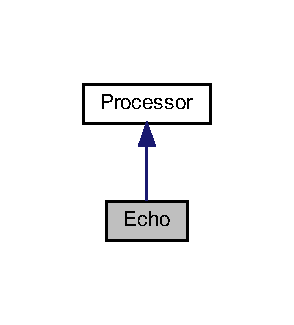
\includegraphics[width=141pt]{d1/dd3/classEcho__inherit__graph}
\end{center}
\end{figure}


Collaboration diagram for Echo\+:
\nopagebreak
\begin{figure}[H]
\begin{center}
\leavevmode
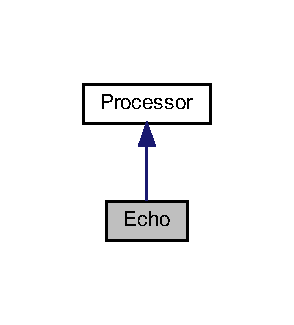
\includegraphics[width=141pt]{da/d44/classEcho__coll__graph}
\end{center}
\end{figure}
\subsection*{Public Member Functions}
\begin{DoxyCompactItemize}
\item 
\mbox{\Hypertarget{classEcho_a28d71de619dda9e6e51567a04bfb60d6}\label{classEcho_a28d71de619dda9e6e51567a04bfb60d6}} 
{\bfseries Echo} (int new\+Delay)
\item 
void \hyperlink{classEcho_ae915d9d4065a34411d18791a5ae9006b}{process\+Buffer} (unsigned char $\ast$buffer, int buffer\+Size) override
\begin{DoxyCompactList}\small\item\em This function creates delayed signals, each one with less amplitude than the one before. \end{DoxyCompactList}\item 
void \hyperlink{classEcho_a3c62f947fd0f9ef063269ed2ca4fab8e}{process\+Buffer} (signed short $\ast$buffer, int buffer\+Size) override
\begin{DoxyCompactList}\small\item\em This function creates delayed signals, each one with less amplitude than the one before. \end{DoxyCompactList}\item 
void \hyperlink{classEcho_ab2dcc623d727179be1dcb8ac34a8453b}{process\+Stereo\+Buffer} (unsigned char $\ast$buffer, int buffer\+Size) override
\begin{DoxyCompactList}\small\item\em For each of the left and right signals of the buffer of the stereo audio file, this function creates delayed signals, each one with less amplitude than the one before. \end{DoxyCompactList}\item 
void \hyperlink{classEcho_a20e6822ef9fc01f0afec9cb8b890a70c}{process\+Stereo\+Buffer} (signed short $\ast$buffer, int buffer\+Size) override
\begin{DoxyCompactList}\small\item\em For each of the left and right signals of the buffer of the stereo audio file, this function creates delayed signals, each one with less amplitude than the one before. \end{DoxyCompactList}\end{DoxyCompactItemize}


\subsection{Member Function Documentation}
\mbox{\Hypertarget{classEcho_ae915d9d4065a34411d18791a5ae9006b}\label{classEcho_ae915d9d4065a34411d18791a5ae9006b}} 
\index{Echo@{Echo}!process\+Buffer@{process\+Buffer}}
\index{process\+Buffer@{process\+Buffer}!Echo@{Echo}}
\subsubsection{\texorpdfstring{process\+Buffer()}{processBuffer()}\hspace{0.1cm}{\footnotesize\ttfamily [1/2]}}
{\footnotesize\ttfamily void Echo\+::process\+Buffer (\begin{DoxyParamCaption}\item[{unsigned char $\ast$}]{buffer,  }\item[{int}]{buffer\+Size }\end{DoxyParamCaption})\hspace{0.3cm}{\ttfamily [override]}, {\ttfamily [virtual]}}



This function creates delayed signals, each one with less amplitude than the one before. 


\begin{DoxyParams}{Parameters}
{\em buffer} & unsigned char$\ast$ buffer of the audio signals for 8 bit mono audio file \\
\hline
{\em buffer\+Size} & \\
\hline
\end{DoxyParams}


Implements \hyperlink{classProcessor}{Processor}.

\mbox{\Hypertarget{classEcho_a3c62f947fd0f9ef063269ed2ca4fab8e}\label{classEcho_a3c62f947fd0f9ef063269ed2ca4fab8e}} 
\index{Echo@{Echo}!process\+Buffer@{process\+Buffer}}
\index{process\+Buffer@{process\+Buffer}!Echo@{Echo}}
\subsubsection{\texorpdfstring{process\+Buffer()}{processBuffer()}\hspace{0.1cm}{\footnotesize\ttfamily [2/2]}}
{\footnotesize\ttfamily void Echo\+::process\+Buffer (\begin{DoxyParamCaption}\item[{signed short $\ast$}]{buffer,  }\item[{int}]{buffer\+Size }\end{DoxyParamCaption})\hspace{0.3cm}{\ttfamily [override]}, {\ttfamily [virtual]}}



This function creates delayed signals, each one with less amplitude than the one before. 


\begin{DoxyParams}{Parameters}
{\em buffer} & signed short$\ast$ buffer of the audio signals for a 16 bit mono audio file \\
\hline
{\em buffer\+Size} & \\
\hline
\end{DoxyParams}


Implements \hyperlink{classProcessor}{Processor}.

\mbox{\Hypertarget{classEcho_ab2dcc623d727179be1dcb8ac34a8453b}\label{classEcho_ab2dcc623d727179be1dcb8ac34a8453b}} 
\index{Echo@{Echo}!process\+Stereo\+Buffer@{process\+Stereo\+Buffer}}
\index{process\+Stereo\+Buffer@{process\+Stereo\+Buffer}!Echo@{Echo}}
\subsubsection{\texorpdfstring{process\+Stereo\+Buffer()}{processStereoBuffer()}\hspace{0.1cm}{\footnotesize\ttfamily [1/2]}}
{\footnotesize\ttfamily void Echo\+::process\+Stereo\+Buffer (\begin{DoxyParamCaption}\item[{unsigned char $\ast$}]{buffer,  }\item[{int}]{buffer\+Size }\end{DoxyParamCaption})\hspace{0.3cm}{\ttfamily [override]}, {\ttfamily [virtual]}}



For each of the left and right signals of the buffer of the stereo audio file, this function creates delayed signals, each one with less amplitude than the one before. 


\begin{DoxyParams}{Parameters}
{\em buffer} & unsigned char$\ast$ buffer of the audio signals for 8 bit stereo audio file \\
\hline
{\em buffer\+Size} & \\
\hline
\end{DoxyParams}


Implements \hyperlink{classProcessor}{Processor}.

\mbox{\Hypertarget{classEcho_a20e6822ef9fc01f0afec9cb8b890a70c}\label{classEcho_a20e6822ef9fc01f0afec9cb8b890a70c}} 
\index{Echo@{Echo}!process\+Stereo\+Buffer@{process\+Stereo\+Buffer}}
\index{process\+Stereo\+Buffer@{process\+Stereo\+Buffer}!Echo@{Echo}}
\subsubsection{\texorpdfstring{process\+Stereo\+Buffer()}{processStereoBuffer()}\hspace{0.1cm}{\footnotesize\ttfamily [2/2]}}
{\footnotesize\ttfamily void Echo\+::process\+Stereo\+Buffer (\begin{DoxyParamCaption}\item[{signed short $\ast$}]{buffer,  }\item[{int}]{buffer\+Size }\end{DoxyParamCaption})\hspace{0.3cm}{\ttfamily [override]}, {\ttfamily [virtual]}}



For each of the left and right signals of the buffer of the stereo audio file, this function creates delayed signals, each one with less amplitude than the one before. 


\begin{DoxyParams}{Parameters}
{\em buffer} & signed short$\ast$ buffer of the audio signals for a 16 bit stereo audio file \\
\hline
{\em buffer\+Size} & \\
\hline
\end{DoxyParams}


Implements \hyperlink{classProcessor}{Processor}.



The documentation for this class was generated from the following files\+:\begin{DoxyCompactItemize}
\item 
Echo.\+h\item 
Echo.\+cpp\end{DoxyCompactItemize}

\hypertarget{classIReadable}{}\section{I\+Readable Class Reference}
\label{classIReadable}\index{I\+Readable@{I\+Readable}}


Inheritance diagram for I\+Readable\+:
\nopagebreak
\begin{figure}[H]
\begin{center}
\leavevmode
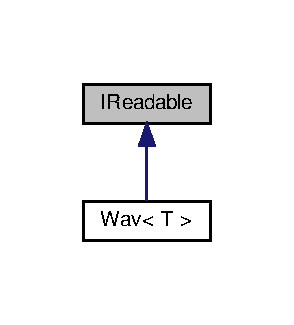
\includegraphics[width=141pt]{d9/d24/classIReadable__inherit__graph}
\end{center}
\end{figure}
\subsection*{Public Member Functions}
\begin{DoxyCompactItemize}
\item 
\mbox{\Hypertarget{classIReadable_a0ed44957150b8cd8becce0f929547b8b}\label{classIReadable_a0ed44957150b8cd8becce0f929547b8b}} 
virtual void {\bfseries read\+File} (const std\+::string \&filename)=0
\end{DoxyCompactItemize}


The documentation for this class was generated from the following file\+:\begin{DoxyCompactItemize}
\item 
I\+Readable.\+h\end{DoxyCompactItemize}

\hypertarget{classlibprocessor}{}\section{libprocessor Class Reference}
\label{classlibprocessor}\index{libprocessor@{libprocessor}}
\subsection*{Public Member Functions}
\begin{DoxyCompactItemize}
\item 
\mbox{\Hypertarget{classlibprocessor_ac22855913d8d2ed6e23760382be25268}\label{classlibprocessor_ac22855913d8d2ed6e23760382be25268}} 
virtual void {\bfseries process\+Buffer} (unsigned char $\ast$buffer, int buffer\+Size)=0
\item 
\mbox{\Hypertarget{classlibprocessor_af4145468e45eabe4f0a7400a1d872832}\label{classlibprocessor_af4145468e45eabe4f0a7400a1d872832}} 
virtual void {\bfseries process\+Buffer} (signed short $\ast$buffer, int buffer\+Size)=0
\item 
\mbox{\Hypertarget{classlibprocessor_aa93ae2a6e1fe55a6a610cd6cfdc85c5c}\label{classlibprocessor_aa93ae2a6e1fe55a6a610cd6cfdc85c5c}} 
virtual void {\bfseries process\+Stereo\+Buffer} (unsigned char $\ast$buffer, int buffer\+Size)=0
\item 
\mbox{\Hypertarget{classlibprocessor_a509704575cda1d6cc317842d1f19bbeb}\label{classlibprocessor_a509704575cda1d6cc317842d1f19bbeb}} 
virtual void {\bfseries process\+Stereo\+Buffer} (signed short $\ast$buffer, int buffer\+Size)=0
\end{DoxyCompactItemize}


The documentation for this class was generated from the following file\+:\begin{DoxyCompactItemize}
\item 
libprocessors.\+h\end{DoxyCompactItemize}

\hypertarget{structList}{}\section{List Struct Reference}
\label{structList}\index{List@{List}}
\subsection*{Public Attributes}
\begin{DoxyCompactItemize}
\item 
\mbox{\Hypertarget{structList_a11c192d98d4c47a4464957d57706cded}\label{structList_a11c192d98d4c47a4464957d57706cded}} 
char {\bfseries info\+ID} \mbox{[}4\mbox{]}
\item 
\mbox{\Hypertarget{structList_af66bdb027f2f2679d8a12223e1ba1380}\label{structList_af66bdb027f2f2679d8a12223e1ba1380}} 
int {\bfseries info\+Size}
\item 
\mbox{\Hypertarget{structList_adf58df5ffd32a14eca080005f2ef6320}\label{structList_adf58df5ffd32a14eca080005f2ef6320}} 
char $\ast$ {\bfseries info}
\end{DoxyCompactItemize}


The documentation for this struct was generated from the following file\+:\begin{DoxyCompactItemize}
\item 
List.\+h\end{DoxyCompactItemize}

\hypertarget{structListHeader}{}\section{List\+Header Struct Reference}
\label{structListHeader}\index{List\+Header@{List\+Header}}
\subsection*{Public Attributes}
\begin{DoxyCompactItemize}
\item 
\mbox{\Hypertarget{structListHeader_a6de963dff7ecaa24b7dd16cef513bb9c}\label{structListHeader_a6de963dff7ecaa24b7dd16cef513bb9c}} 
char {\bfseries L\+I\+ST} \mbox{[}4\mbox{]}
\item 
\mbox{\Hypertarget{structListHeader_a4f347f9e217e8bc0723975ecd7975282}\label{structListHeader_a4f347f9e217e8bc0723975ecd7975282}} 
int {\bfseries list\+Chunk\+Size}
\item 
\mbox{\Hypertarget{structListHeader_a8a4260170092fefe13be38605ef2e239}\label{structListHeader_a8a4260170092fefe13be38605ef2e239}} 
char {\bfseries type\+ID} \mbox{[}4\mbox{]}
\end{DoxyCompactItemize}


The documentation for this struct was generated from the following file\+:\begin{DoxyCompactItemize}
\item 
List\+Header.\+h\end{DoxyCompactItemize}

\hypertarget{classModify}{}\section{Modify Class Reference}
\label{classModify}\index{Modify@{Modify}}
\subsection*{Public Member Functions}
\begin{DoxyCompactItemize}
\item 
\hyperlink{structList}{List} $\ast$ \hyperlink{classModify_a7687f4996264b9dee1ac335856be7be4}{modify\+Metadata} (\hyperlink{structList}{List} $\ast$metadata\+Obj, std\+::string new\+Metadata\+String)
\begin{DoxyCompactList}\small\item\em This function modifies data of specified list object to user\textquotesingle{}s input and updates the corresponding data length. \end{DoxyCompactList}\item 
\mbox{\Hypertarget{classModify_aa7f1bf33dbcb800828d846edeb35fc56}\label{classModify_aa7f1bf33dbcb800828d846edeb35fc56}} 
void {\bfseries add\+Metadata\+Section} (std\+::vector$<$ \hyperlink{structList}{List} $>$ list, char new\+Info\+ID\mbox{[}4\mbox{]}, std\+::string new\+Info)
\end{DoxyCompactItemize}


\subsection{Member Function Documentation}
\mbox{\Hypertarget{classModify_a7687f4996264b9dee1ac335856be7be4}\label{classModify_a7687f4996264b9dee1ac335856be7be4}} 
\index{Modify@{Modify}!modify\+Metadata@{modify\+Metadata}}
\index{modify\+Metadata@{modify\+Metadata}!Modify@{Modify}}
\subsubsection{\texorpdfstring{modify\+Metadata()}{modifyMetadata()}}
{\footnotesize\ttfamily \hyperlink{structList}{List} $\ast$ Modify\+::modify\+Metadata (\begin{DoxyParamCaption}\item[{\hyperlink{structList}{List} $\ast$}]{metadata\+Obj,  }\item[{std\+::string}]{new\+Metadata\+String }\end{DoxyParamCaption})}



This function modifies data of specified list object to user\textquotesingle{}s input and updates the corresponding data length. 


\begin{DoxyParams}{Parameters}
{\em metadata\+Obj} & object that will be modified \\
\hline
{\em new\+Metadata\+String} & User Input \\
\hline
\end{DoxyParams}


The documentation for this class was generated from the following files\+:\begin{DoxyCompactItemize}
\item 
Modify.\+h\item 
Modify.\+cpp\end{DoxyCompactItemize}

\hypertarget{classNoiseGate}{}\section{Noise\+Gate Class Reference}
\label{classNoiseGate}\index{Noise\+Gate@{Noise\+Gate}}


Inheritance diagram for Noise\+Gate\+:
\nopagebreak
\begin{figure}[H]
\begin{center}
\leavevmode
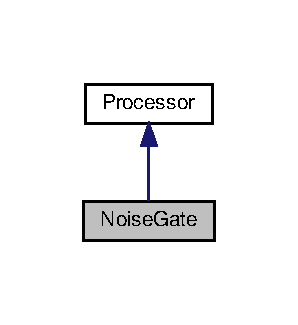
\includegraphics[width=143pt]{d5/d39/classNoiseGate__inherit__graph}
\end{center}
\end{figure}


Collaboration diagram for Noise\+Gate\+:
\nopagebreak
\begin{figure}[H]
\begin{center}
\leavevmode
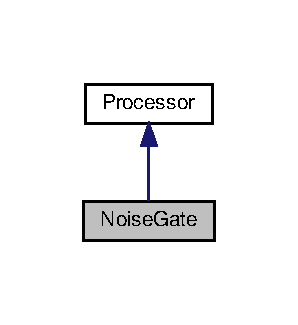
\includegraphics[width=143pt]{d8/da9/classNoiseGate__coll__graph}
\end{center}
\end{figure}
\subsection*{Public Member Functions}
\begin{DoxyCompactItemize}
\item 
\mbox{\Hypertarget{classNoiseGate_aecd2507a2de086259c70047c2fdcbb28}\label{classNoiseGate_aecd2507a2de086259c70047c2fdcbb28}} 
{\bfseries Noise\+Gate} (float new\+Threshold)
\item 
void \hyperlink{classNoiseGate_acab8baa73ab66ee5c377631c2c1f3c72}{process\+Buffer} (unsigned char $\ast$buffer, int buffer\+Size) override
\begin{DoxyCompactList}\small\item\em This function sets any signals that fall within the threshold area to 0. \end{DoxyCompactList}\item 
void \hyperlink{classNoiseGate_a7fff3386cd56cb96c60ccec17ec6afd0}{process\+Buffer} (signed short $\ast$buffer, int buffer\+Size) override
\begin{DoxyCompactList}\small\item\em This function sets any signals that fall within the threshold area to 0. \end{DoxyCompactList}\item 
void \hyperlink{classNoiseGate_aeb214c7a4183ee24ef073a3e5c029f94}{process\+Stereo\+Buffer} (unsigned char $\ast$buffer, int buffer\+Size) override
\begin{DoxyCompactList}\small\item\em For each of the left and right signals of the buffer in the stereo file, this function sets any signals that fall within the threshold area to 0. \end{DoxyCompactList}\item 
void \hyperlink{classNoiseGate_a95327c88365a0371c127b9c63bbe56bc}{process\+Stereo\+Buffer} (signed short $\ast$buffer, int buffer\+Size) override
\begin{DoxyCompactList}\small\item\em For each of the left and right signals of the buffer in the stereo audio file, this function sets any signals that fall within the threshold area to 0. \end{DoxyCompactList}\end{DoxyCompactItemize}


\subsection{Member Function Documentation}
\mbox{\Hypertarget{classNoiseGate_acab8baa73ab66ee5c377631c2c1f3c72}\label{classNoiseGate_acab8baa73ab66ee5c377631c2c1f3c72}} 
\index{Noise\+Gate@{Noise\+Gate}!process\+Buffer@{process\+Buffer}}
\index{process\+Buffer@{process\+Buffer}!Noise\+Gate@{Noise\+Gate}}
\subsubsection{\texorpdfstring{process\+Buffer()}{processBuffer()}\hspace{0.1cm}{\footnotesize\ttfamily [1/2]}}
{\footnotesize\ttfamily void Noise\+Gate\+::process\+Buffer (\begin{DoxyParamCaption}\item[{unsigned char $\ast$}]{buffer,  }\item[{int}]{buffer\+Size }\end{DoxyParamCaption})\hspace{0.3cm}{\ttfamily [override]}, {\ttfamily [virtual]}}



This function sets any signals that fall within the threshold area to 0. 


\begin{DoxyParams}{Parameters}
{\em buffer} & unsigned char$\ast$ buffer of the audio signals for 8 bit mono audio file \\
\hline
{\em buffer\+Size} & \\
\hline
\end{DoxyParams}


Implements \hyperlink{classProcessor}{Processor}.

\mbox{\Hypertarget{classNoiseGate_a7fff3386cd56cb96c60ccec17ec6afd0}\label{classNoiseGate_a7fff3386cd56cb96c60ccec17ec6afd0}} 
\index{Noise\+Gate@{Noise\+Gate}!process\+Buffer@{process\+Buffer}}
\index{process\+Buffer@{process\+Buffer}!Noise\+Gate@{Noise\+Gate}}
\subsubsection{\texorpdfstring{process\+Buffer()}{processBuffer()}\hspace{0.1cm}{\footnotesize\ttfamily [2/2]}}
{\footnotesize\ttfamily void Noise\+Gate\+::process\+Buffer (\begin{DoxyParamCaption}\item[{signed short $\ast$}]{buffer,  }\item[{int}]{buffer\+Size }\end{DoxyParamCaption})\hspace{0.3cm}{\ttfamily [override]}, {\ttfamily [virtual]}}



This function sets any signals that fall within the threshold area to 0. 


\begin{DoxyParams}{Parameters}
{\em buffer} & signed short$\ast$ buffer of the audio signals for a 16 bit mono audio file \\
\hline
{\em buffer\+Size} & \\
\hline
\end{DoxyParams}


Implements \hyperlink{classProcessor}{Processor}.

\mbox{\Hypertarget{classNoiseGate_aeb214c7a4183ee24ef073a3e5c029f94}\label{classNoiseGate_aeb214c7a4183ee24ef073a3e5c029f94}} 
\index{Noise\+Gate@{Noise\+Gate}!process\+Stereo\+Buffer@{process\+Stereo\+Buffer}}
\index{process\+Stereo\+Buffer@{process\+Stereo\+Buffer}!Noise\+Gate@{Noise\+Gate}}
\subsubsection{\texorpdfstring{process\+Stereo\+Buffer()}{processStereoBuffer()}\hspace{0.1cm}{\footnotesize\ttfamily [1/2]}}
{\footnotesize\ttfamily void Noise\+Gate\+::process\+Stereo\+Buffer (\begin{DoxyParamCaption}\item[{unsigned char $\ast$}]{buffer,  }\item[{int}]{buffer\+Size }\end{DoxyParamCaption})\hspace{0.3cm}{\ttfamily [override]}, {\ttfamily [virtual]}}



For each of the left and right signals of the buffer in the stereo file, this function sets any signals that fall within the threshold area to 0. 


\begin{DoxyParams}{Parameters}
{\em buffer} & unsigned char$\ast$ buffer of the audio signals for 8 bit stereo audio file \\
\hline
{\em buffer\+Size} & \\
\hline
\end{DoxyParams}


Implements \hyperlink{classProcessor}{Processor}.

\mbox{\Hypertarget{classNoiseGate_a95327c88365a0371c127b9c63bbe56bc}\label{classNoiseGate_a95327c88365a0371c127b9c63bbe56bc}} 
\index{Noise\+Gate@{Noise\+Gate}!process\+Stereo\+Buffer@{process\+Stereo\+Buffer}}
\index{process\+Stereo\+Buffer@{process\+Stereo\+Buffer}!Noise\+Gate@{Noise\+Gate}}
\subsubsection{\texorpdfstring{process\+Stereo\+Buffer()}{processStereoBuffer()}\hspace{0.1cm}{\footnotesize\ttfamily [2/2]}}
{\footnotesize\ttfamily void Noise\+Gate\+::process\+Stereo\+Buffer (\begin{DoxyParamCaption}\item[{signed short $\ast$}]{buffer,  }\item[{int}]{buffer\+Size }\end{DoxyParamCaption})\hspace{0.3cm}{\ttfamily [override]}, {\ttfamily [virtual]}}



For each of the left and right signals of the buffer in the stereo audio file, this function sets any signals that fall within the threshold area to 0. 


\begin{DoxyParams}{Parameters}
{\em buffer} & signed short$\ast$ buffer of the audio signals for a 16 bit stereo audio file \\
\hline
{\em buffer\+Size} & \\
\hline
\end{DoxyParams}


Implements \hyperlink{classProcessor}{Processor}.



The documentation for this class was generated from the following files\+:\begin{DoxyCompactItemize}
\item 
Noise\+Gate.\+h\item 
Noise\+Gate.\+cpp\end{DoxyCompactItemize}

\hypertarget{classNormalization}{}\section{Normalization Class Reference}
\label{classNormalization}\index{Normalization@{Normalization}}


Inheritance diagram for Normalization\+:
\nopagebreak
\begin{figure}[H]
\begin{center}
\leavevmode
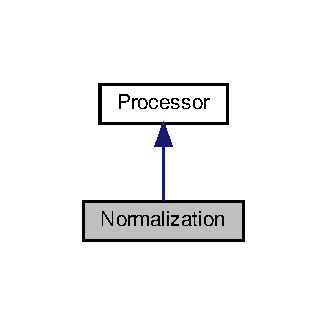
\includegraphics[width=157pt]{d2/d5e/classNormalization__inherit__graph}
\end{center}
\end{figure}


Collaboration diagram for Normalization\+:
\nopagebreak
\begin{figure}[H]
\begin{center}
\leavevmode
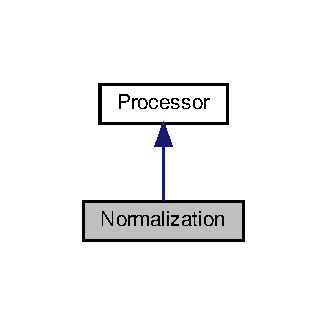
\includegraphics[width=157pt]{de/d74/classNormalization__coll__graph}
\end{center}
\end{figure}
\subsection*{Additional Inherited Members}


The documentation for this class was generated from the following files\+:\begin{DoxyCompactItemize}
\item 
Normalization.\+h\item 
Normalization.\+cpp\end{DoxyCompactItemize}

\hypertarget{classProcessor}{}\section{Processor Class Reference}
\label{classProcessor}\index{Processor@{Processor}}


Inheritance diagram for Processor\+:
\nopagebreak
\begin{figure}[H]
\begin{center}
\leavevmode
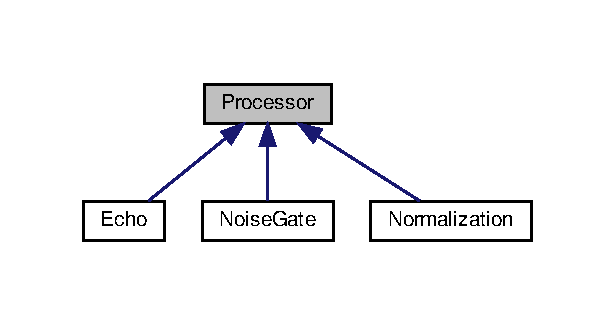
\includegraphics[width=295pt]{dd/d93/classProcessor__inherit__graph}
\end{center}
\end{figure}
\subsection*{Public Member Functions}
\begin{DoxyCompactItemize}
\item 
\mbox{\Hypertarget{classProcessor_a401e57b59e43de9c4a51ca0f566d2948}\label{classProcessor_a401e57b59e43de9c4a51ca0f566d2948}} 
virtual void {\bfseries process\+Buffer} (unsigned char $\ast$buffer, int buffer\+Size)=0
\item 
\mbox{\Hypertarget{classProcessor_a43c891cf4889858380375c455e02df45}\label{classProcessor_a43c891cf4889858380375c455e02df45}} 
virtual void {\bfseries process\+Buffer} (signed short $\ast$buffer, int buffer\+Size)=0
\item 
\mbox{\Hypertarget{classProcessor_a06ecb7c9959d197a363f5ff4c33c6eb3}\label{classProcessor_a06ecb7c9959d197a363f5ff4c33c6eb3}} 
virtual void {\bfseries process\+Stereo\+Buffer} (unsigned char $\ast$buffer, int buffer\+Size)=0
\item 
\mbox{\Hypertarget{classProcessor_adf8eed92a112cee827466f0ca93cce93}\label{classProcessor_adf8eed92a112cee827466f0ca93cce93}} 
virtual void {\bfseries process\+Stereo\+Buffer} (signed short $\ast$buffer, int buffer\+Size)=0
\end{DoxyCompactItemize}


The documentation for this class was generated from the following file\+:\begin{DoxyCompactItemize}
\item 
Processor.\+h\end{DoxyCompactItemize}

\hypertarget{classWav}{}\section{Wav$<$ T $>$ Class Template Reference}
\label{classWav}\index{Wav$<$ T $>$@{Wav$<$ T $>$}}


{\ttfamily \#include $<$Wav.\+h$>$}



Inheritance diagram for Wav$<$ T $>$\+:
\nopagebreak
\begin{figure}[H]
\begin{center}
\leavevmode
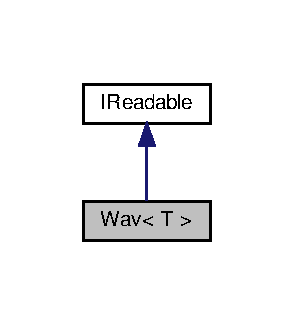
\includegraphics[width=141pt]{d1/d86/classWav__inherit__graph}
\end{center}
\end{figure}


Collaboration diagram for Wav$<$ T $>$\+:
\nopagebreak
\begin{figure}[H]
\begin{center}
\leavevmode
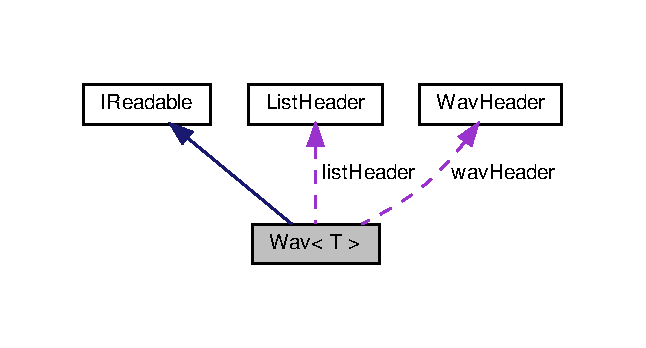
\includegraphics[width=310pt]{db/dac/classWav__coll__graph}
\end{center}
\end{figure}
\subsection*{Public Member Functions}
\begin{DoxyCompactItemize}
\item 
\hyperlink{classWav_ab265f0e3e012960f531ed5ff242c4e52}{Wav} (std\+::string in\+File)
\begin{DoxyCompactList}\small\item\em Constructor for the \hyperlink{classWav}{Wav} class. \end{DoxyCompactList}\item 
void \hyperlink{classWav_a636a94bf0f23a4cdc9d8d59d9d567f3e}{read\+File} (const std\+::string \&filename) override
\begin{DoxyCompactList}\small\item\em Function to read data from an inputted .wav file. \end{DoxyCompactList}\item 
void \hyperlink{classWav_afbae07371a8e0f17cc8e3a29507016e3}{write\+File} (const std\+::string \&out\+File\+Name)
\begin{DoxyCompactList}\small\item\em Function to write data to a wav file. \end{DoxyCompactList}\item 
\mbox{\Hypertarget{classWav_ae484d2f0d2ce244ed23b99be6ea43977}\label{classWav_ae484d2f0d2ce244ed23b99be6ea43977}} 
bool \hyperlink{classWav_ae484d2f0d2ce244ed23b99be6ea43977}{check\+For\+List} ()
\begin{DoxyCompactList}\small\item\em Determines if the wav file has a \hyperlink{structList}{List} subchunk. \end{DoxyCompactList}\item 
\mbox{\Hypertarget{classWav_afd1ee6d72bb1bac1284a0df3ae7d9cea}\label{classWav_afd1ee6d72bb1bac1284a0df3ae7d9cea}} 
int \hyperlink{classWav_afd1ee6d72bb1bac1284a0df3ae7d9cea}{get\+Buffer\+Size} () const
\begin{DoxyCompactList}\small\item\em Returns the size of the data buffer in bytes. \end{DoxyCompactList}\item 
\mbox{\Hypertarget{classWav_adc3bc9bcc037ff83bc7544715e70e144}\label{classWav_adc3bc9bcc037ff83bc7544715e70e144}} 
T $\ast$ \hyperlink{classWav_adc3bc9bcc037ff83bc7544715e70e144}{get\+Buffer} () const
\begin{DoxyCompactList}\small\item\em Returns a pointer to the data buffer. \end{DoxyCompactList}\item 
\mbox{\Hypertarget{classWav_ad974c0f10e70e23d689d60591aa90456}\label{classWav_ad974c0f10e70e23d689d60591aa90456}} 
std\+::vector$<$ \hyperlink{structList}{List} $>$ \hyperlink{classWav_ad974c0f10e70e23d689d60591aa90456}{get\+List\+Vector} () const
\begin{DoxyCompactList}\small\item\em Returns the vector of \hyperlink{structList}{List} objects. \end{DoxyCompactList}\item 
virtual \hyperlink{classWav_a54ee39542f46929187c7a9e032250bdf}{$\sim$\+Wav} ()
\end{DoxyCompactItemize}
\subsection*{Public Attributes}
\begin{DoxyCompactItemize}
\item 
\mbox{\Hypertarget{classWav_afc68f75eb85a46db0a63971974f8d5be}\label{classWav_afc68f75eb85a46db0a63971974f8d5be}} 
\hyperlink{structWavHeader}{Wav\+Header} {\bfseries wav\+Header}
\item 
\mbox{\Hypertarget{classWav_a89f07c2c8726afdffb8139842a9af064}\label{classWav_a89f07c2c8726afdffb8139842a9af064}} 
\hyperlink{structListHeader}{List\+Header} {\bfseries list\+Header}
\item 
\mbox{\Hypertarget{classWav_addc4d0d2a45357e8f981e4979c54b91a}\label{classWav_addc4d0d2a45357e8f981e4979c54b91a}} 
bool {\bfseries has\+List\+Chunk} = 0
\item 
\mbox{\Hypertarget{classWav_a5533801d7288f0f5aad06b032421e9c1}\label{classWav_a5533801d7288f0f5aad06b032421e9c1}} 
std\+::vector$<$ \hyperlink{structList}{List} $>$ {\bfseries list}
\item 
\mbox{\Hypertarget{classWav_a329a81309898a70392426f69df63ddaa}\label{classWav_a329a81309898a70392426f69df63ddaa}} 
T $\ast$ {\bfseries buffer} = N\+U\+LL
\item 
\mbox{\Hypertarget{classWav_a75e9243abb294e0a69633b3dd8d7adbb}\label{classWav_a75e9243abb294e0a69633b3dd8d7adbb}} 
std\+::string {\bfseries in\+File}
\end{DoxyCompactItemize}


\subsection{Detailed Description}
\subsubsection*{template$<$typename T$>$\newline
class Wav$<$ T $>$}

This is the \hyperlink{classWav}{Wav} class. It is templatized so that it will accept data buffers of type short for 16 bit wav files or unsigned char for 8 bit wav files 

\subsection{Constructor \& Destructor Documentation}
\mbox{\Hypertarget{classWav_ab265f0e3e012960f531ed5ff242c4e52}\label{classWav_ab265f0e3e012960f531ed5ff242c4e52}} 
\index{Wav@{Wav}!Wav@{Wav}}
\index{Wav@{Wav}!Wav@{Wav}}
\subsubsection{\texorpdfstring{Wav()}{Wav()}}
{\footnotesize\ttfamily template$<$typename T $>$ \\
\hyperlink{classWav}{Wav}$<$ T $>$\+::\hyperlink{classWav}{Wav} (\begin{DoxyParamCaption}\item[{std\+::string}]{in\+File }\end{DoxyParamCaption})}



Constructor for the \hyperlink{classWav}{Wav} class. 


\begin{DoxyParams}{Parameters}
{\em in\+File} & -\/ name of the .wav file being read from \\
\hline
\end{DoxyParams}
\mbox{\Hypertarget{classWav_a54ee39542f46929187c7a9e032250bdf}\label{classWav_a54ee39542f46929187c7a9e032250bdf}} 
\index{Wav@{Wav}!````~Wav@{$\sim$\+Wav}}
\index{````~Wav@{$\sim$\+Wav}!Wav@{Wav}}
\subsubsection{\texorpdfstring{$\sim$\+Wav()}{~Wav()}}
{\footnotesize\ttfamily template$<$typename T $>$ \\
virtual \hyperlink{classWav}{Wav}$<$ T $>$\+::$\sim$\hyperlink{classWav}{Wav} (\begin{DoxyParamCaption}{ }\end{DoxyParamCaption})\hspace{0.3cm}{\ttfamily [inline]}, {\ttfamily [virtual]}}

Destructor for the \hyperlink{classWav}{Wav} class that deletes the buffer if it is not empty 

\subsection{Member Function Documentation}
\mbox{\Hypertarget{classWav_a636a94bf0f23a4cdc9d8d59d9d567f3e}\label{classWav_a636a94bf0f23a4cdc9d8d59d9d567f3e}} 
\index{Wav@{Wav}!read\+File@{read\+File}}
\index{read\+File@{read\+File}!Wav@{Wav}}
\subsubsection{\texorpdfstring{read\+File()}{readFile()}}
{\footnotesize\ttfamily template$<$typename T $>$ \\
void \hyperlink{classWav}{Wav}$<$ T $>$\+::read\+File (\begin{DoxyParamCaption}\item[{const std\+::string \&}]{filename }\end{DoxyParamCaption})\hspace{0.3cm}{\ttfamily [override]}, {\ttfamily [virtual]}}



Function to read data from an inputted .wav file. 


\begin{DoxyParams}{Parameters}
{\em filename} & -\/ the name of the .wav file being read from; overrides from \hyperlink{classIReadable}{I\+Readable} \\
\hline
\end{DoxyParams}


Implements \hyperlink{classIReadable}{I\+Readable}.

\mbox{\Hypertarget{classWav_afbae07371a8e0f17cc8e3a29507016e3}\label{classWav_afbae07371a8e0f17cc8e3a29507016e3}} 
\index{Wav@{Wav}!write\+File@{write\+File}}
\index{write\+File@{write\+File}!Wav@{Wav}}
\subsubsection{\texorpdfstring{write\+File()}{writeFile()}}
{\footnotesize\ttfamily template$<$typename T $>$ \\
void \hyperlink{classWav}{Wav}$<$ T $>$\+::write\+File (\begin{DoxyParamCaption}\item[{const std\+::string \&}]{out\+File\+Name }\end{DoxyParamCaption})}



Function to write data to a wav file. 


\begin{DoxyParams}{Parameters}
{\em out\+File\+Name} & -\/ the name of the .wav file being written to \\
\hline
\end{DoxyParams}


The documentation for this class was generated from the following files\+:\begin{DoxyCompactItemize}
\item 
Wav.\+h\item 
Wav.\+cpp\end{DoxyCompactItemize}

\hypertarget{classWavConsole}{}\section{Wav\+Console Class Reference}
\label{classWavConsole}\index{Wav\+Console@{Wav\+Console}}


Collaboration diagram for Wav\+Console\+:
\nopagebreak
\begin{figure}[H]
\begin{center}
\leavevmode
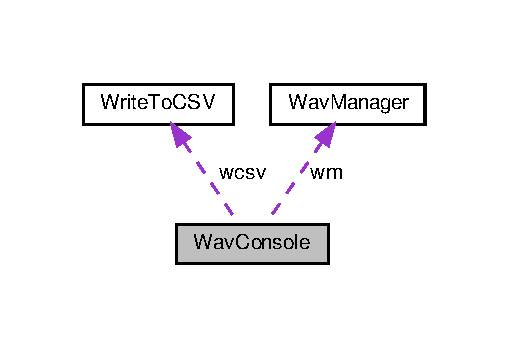
\includegraphics[width=244pt]{de/dee/classWavConsole__coll__graph}
\end{center}
\end{figure}
\subsection*{Public Member Functions}
\begin{DoxyCompactItemize}
\item 
void \hyperlink{classWavConsole_af15680c1257375a6f687ad5c4c0b9b0c}{add\+Command} (std\+::string name, std\+::string help\+Text)
\begin{DoxyCompactList}\small\item\em This function pushes a new command to the vector of commands. \end{DoxyCompactList}\item 
\mbox{\Hypertarget{classWavConsole_aef531f754faaa5592d78e15e46feb768}\label{classWavConsole_aef531f754faaa5592d78e15e46feb768}} 
void \hyperlink{classWavConsole_aef531f754faaa5592d78e15e46feb768}{print\+Commands} ()
\begin{DoxyCompactList}\small\item\em This function prints the name of each valid console command to show the user what options are available. \end{DoxyCompactList}\item 
std\+::vector$<$ std\+::experimental\+::filesystem\+::path $>$ \hyperlink{classWavConsole_ae5ee40c484223159f58d2758c0dba340}{pull\+Filenames} (std\+::string directory)
\begin{DoxyCompactList}\small\item\em This function uses a directory\+\_\+iterator to get the names of every file in the user-\/inputted directory. \end{DoxyCompactList}\item 
\mbox{\Hypertarget{classWavConsole_af1b08107ff8d69c7515d719b7b88a164}\label{classWavConsole_af1b08107ff8d69c7515d719b7b88a164}} 
void \hyperlink{classWavConsole_af1b08107ff8d69c7515d719b7b88a164}{run\+Console} ()
\begin{DoxyCompactList}\small\item\em This function is the main interface with the user. It guides the user through the use of the W\+AV managment and processing system and calls classes to process, edit, read, and write as required. \end{DoxyCompactList}\end{DoxyCompactItemize}
\subsection*{Public Attributes}
\begin{DoxyCompactItemize}
\item 
\mbox{\Hypertarget{classWavConsole_adcec7b4b592a3b2fa08c566c7a409ac6}\label{classWavConsole_adcec7b4b592a3b2fa08c566c7a409ac6}} 
\hyperlink{classWavManager}{Wav\+Manager} {\bfseries wm}
\item 
\mbox{\Hypertarget{classWavConsole_ac86ec2cd3fa6a3f9ba04dd3fa9e0b804}\label{classWavConsole_ac86ec2cd3fa6a3f9ba04dd3fa9e0b804}} 
\hyperlink{classWriteToCSV}{Write\+To\+C\+SV} {\bfseries wcsv}
\item 
\mbox{\Hypertarget{classWavConsole_a55c09e96cfa25fb73c6dfd963e5f61ef}\label{classWavConsole_a55c09e96cfa25fb73c6dfd963e5f61ef}} 
std\+::vector$<$ \hyperlink{classCommand}{Command} $>$ {\bfseries commands}
\end{DoxyCompactItemize}


\subsection{Member Function Documentation}
\mbox{\Hypertarget{classWavConsole_af15680c1257375a6f687ad5c4c0b9b0c}\label{classWavConsole_af15680c1257375a6f687ad5c4c0b9b0c}} 
\index{Wav\+Console@{Wav\+Console}!add\+Command@{add\+Command}}
\index{add\+Command@{add\+Command}!Wav\+Console@{Wav\+Console}}
\subsubsection{\texorpdfstring{add\+Command()}{addCommand()}}
{\footnotesize\ttfamily void Wav\+Console\+::add\+Command (\begin{DoxyParamCaption}\item[{std\+::string}]{name,  }\item[{std\+::string}]{help\+Text }\end{DoxyParamCaption})}



This function pushes a new command to the vector of commands. 


\begin{DoxyParams}{Parameters}
{\em name} & Name of the chat command. \\
\hline
{\em help\+Text} & Text to display when additional info is requested on the command. \\
\hline
\end{DoxyParams}
\mbox{\Hypertarget{classWavConsole_ae5ee40c484223159f58d2758c0dba340}\label{classWavConsole_ae5ee40c484223159f58d2758c0dba340}} 
\index{Wav\+Console@{Wav\+Console}!pull\+Filenames@{pull\+Filenames}}
\index{pull\+Filenames@{pull\+Filenames}!Wav\+Console@{Wav\+Console}}
\subsubsection{\texorpdfstring{pull\+Filenames()}{pullFilenames()}}
{\footnotesize\ttfamily vector$<$ std\+::experimental\+::filesystem\+::path $>$ Wav\+Console\+::pull\+Filenames (\begin{DoxyParamCaption}\item[{std\+::string}]{directory }\end{DoxyParamCaption})}



This function uses a directory\+\_\+iterator to get the names of every file in the user-\/inputted directory. 


\begin{DoxyParams}{Parameters}
{\em directory} & User-\/inputted path to the directory of W\+A\+Vs to manipulate. \\
\hline
\end{DoxyParams}


The documentation for this class was generated from the following files\+:\begin{DoxyCompactItemize}
\item 
Wav\+Console.\+h\item 
Wav\+Console.\+cpp\end{DoxyCompactItemize}

\hypertarget{structWavHeader}{}\section{Wav\+Header Struct Reference}
\label{structWavHeader}\index{Wav\+Header@{Wav\+Header}}
\subsection*{Public Attributes}
\begin{DoxyCompactItemize}
\item 
\mbox{\Hypertarget{structWavHeader_a656b55f18ceefdc4e7678d77314237bd}\label{structWavHeader_a656b55f18ceefdc4e7678d77314237bd}} 
char {\bfseries R\+I\+FF} \mbox{[}4\mbox{]}
\item 
\mbox{\Hypertarget{structWavHeader_aabec07ac9c8400dfb62e18d23fa6a5c1}\label{structWavHeader_aabec07ac9c8400dfb62e18d23fa6a5c1}} 
int {\bfseries chunk\+Size}
\item 
\mbox{\Hypertarget{structWavHeader_a09588720e7193c0a523da6325bc17a20}\label{structWavHeader_a09588720e7193c0a523da6325bc17a20}} 
char {\bfseries W\+A\+VE} \mbox{[}4\mbox{]}
\item 
\mbox{\Hypertarget{structWavHeader_a06a6b5a7d41312b2e4f7c16edd25a905}\label{structWavHeader_a06a6b5a7d41312b2e4f7c16edd25a905}} 
char {\bfseries F\+MT} \mbox{[}4\mbox{]}
\item 
\mbox{\Hypertarget{structWavHeader_acb4b8069da647f000862e5c90b92225f}\label{structWavHeader_acb4b8069da647f000862e5c90b92225f}} 
int {\bfseries fmt\+Chunk\+Size}
\item 
\mbox{\Hypertarget{structWavHeader_af052ba52da4a1bda137ce0171f3d763e}\label{structWavHeader_af052ba52da4a1bda137ce0171f3d763e}} 
short {\bfseries audio\+Format}
\item 
\mbox{\Hypertarget{structWavHeader_a974f24ee8f6c0f7a6a881b1b5f917bfa}\label{structWavHeader_a974f24ee8f6c0f7a6a881b1b5f917bfa}} 
short {\bfseries num\+Channels}
\item 
\mbox{\Hypertarget{structWavHeader_a70f6545b7646e8f9c2f02118150566d1}\label{structWavHeader_a70f6545b7646e8f9c2f02118150566d1}} 
int {\bfseries sample\+Rate}
\item 
\mbox{\Hypertarget{structWavHeader_ab9c193dd57da1a877cd5193657ed8a75}\label{structWavHeader_ab9c193dd57da1a877cd5193657ed8a75}} 
int {\bfseries byte\+Rate}
\item 
\mbox{\Hypertarget{structWavHeader_a4460bbfc889fbf2e988970fd39127c4c}\label{structWavHeader_a4460bbfc889fbf2e988970fd39127c4c}} 
short {\bfseries block\+Alignment}
\item 
\mbox{\Hypertarget{structWavHeader_a2a501acfa50d22cc01a972367e164a77}\label{structWavHeader_a2a501acfa50d22cc01a972367e164a77}} 
short {\bfseries bit\+Depth}
\item 
\mbox{\Hypertarget{structWavHeader_a91c5bef7c13bca1226828e7ca10547a3}\label{structWavHeader_a91c5bef7c13bca1226828e7ca10547a3}} 
char {\bfseries data\+Header} \mbox{[}4\mbox{]}
\item 
\mbox{\Hypertarget{structWavHeader_a9a984c298b6d88f3097e080f42e9ddc8}\label{structWavHeader_a9a984c298b6d88f3097e080f42e9ddc8}} 
int {\bfseries data\+Chunk\+Size}
\end{DoxyCompactItemize}


The documentation for this struct was generated from the following file\+:\begin{DoxyCompactItemize}
\item 
Wav\+Header.\+h\end{DoxyCompactItemize}

\hypertarget{classWavManager}{}\section{Wav\+Manager Class Reference}
\label{classWavManager}\index{Wav\+Manager@{Wav\+Manager}}


{\ttfamily \#include $<$Wav\+Manager.\+h$>$}

\subsection*{Public Member Functions}
\begin{DoxyCompactItemize}
\item 
void \hyperlink{classWavManager_ad777fbcc1b1fb7185c66d69a66842e02}{populate\+Vector} (std\+::vector$<$ std\+::string $>$ filenames)
\begin{DoxyCompactList}\small\item\em Creates \hyperlink{classWav}{Wav} objects and calls the read function for each file in the filenames vector. \end{DoxyCompactList}\end{DoxyCompactItemize}
\subsection*{Public Attributes}
\begin{DoxyCompactItemize}
\item 
\mbox{\Hypertarget{classWavManager_aa12134771083da849053d1d5a6372d65}\label{classWavManager_aa12134771083da849053d1d5a6372d65}} 
std\+::vector$<$ \hyperlink{classIReadable}{I\+Readable} $\ast$ $>$ {\bfseries wavs}
\end{DoxyCompactItemize}


\subsection{Detailed Description}
This is the \hyperlink{classWavManager}{Wav\+Manager} class 

\subsection{Member Function Documentation}
\mbox{\Hypertarget{classWavManager_ad777fbcc1b1fb7185c66d69a66842e02}\label{classWavManager_ad777fbcc1b1fb7185c66d69a66842e02}} 
\index{Wav\+Manager@{Wav\+Manager}!populate\+Vector@{populate\+Vector}}
\index{populate\+Vector@{populate\+Vector}!Wav\+Manager@{Wav\+Manager}}
\subsubsection{\texorpdfstring{populate\+Vector()}{populateVector()}}
{\footnotesize\ttfamily void Wav\+Manager\+::populate\+Vector (\begin{DoxyParamCaption}\item[{std\+::vector$<$ std\+::string $>$}]{filenames }\end{DoxyParamCaption})}



Creates \hyperlink{classWav}{Wav} objects and calls the read function for each file in the filenames vector. 


\begin{DoxyParams}{Parameters}
{\em filenames} & -\/ vector of names of .wav files \\
\hline
\end{DoxyParams}


The documentation for this class was generated from the following files\+:\begin{DoxyCompactItemize}
\item 
Wav\+Manager.\+h\item 
Wav\+Manager.\+cpp\end{DoxyCompactItemize}

\hypertarget{classWriteToCSV}{}\section{Write\+To\+C\+SV Class Reference}
\label{classWriteToCSV}\index{Write\+To\+C\+SV@{Write\+To\+C\+SV}}
\subsection*{Public Member Functions}
\begin{DoxyCompactItemize}
\item 
bool \hyperlink{classWriteToCSV_ab2b17e10aff8b6abd3267def9e53592e}{write\+Data\+To\+File} (std\+::string C\+S\+Vfile\+\_\+name, std\+::vector$<$ std\+::string $>$ file\+Names, std\+::vector$<$ \hyperlink{classIReadable}{I\+Readable} $\ast$$>$ wav\+Files)
\begin{DoxyCompactList}\small\item\em This function writes the technical information and metadata from the given file into a C\+SV file. \end{DoxyCompactList}\end{DoxyCompactItemize}


\subsection{Member Function Documentation}
\mbox{\Hypertarget{classWriteToCSV_ab2b17e10aff8b6abd3267def9e53592e}\label{classWriteToCSV_ab2b17e10aff8b6abd3267def9e53592e}} 
\index{Write\+To\+C\+SV@{Write\+To\+C\+SV}!write\+Data\+To\+File@{write\+Data\+To\+File}}
\index{write\+Data\+To\+File@{write\+Data\+To\+File}!Write\+To\+C\+SV@{Write\+To\+C\+SV}}
\subsubsection{\texorpdfstring{write\+Data\+To\+File()}{writeDataToFile()}}
{\footnotesize\ttfamily bool Write\+To\+C\+S\+V\+::write\+Data\+To\+File (\begin{DoxyParamCaption}\item[{std\+::string}]{C\+S\+Vfile\+\_\+name,  }\item[{std\+::vector$<$ std\+::string $>$}]{file\+Names,  }\item[{std\+::vector$<$ \hyperlink{classIReadable}{I\+Readable} $\ast$$>$}]{wav\+Files }\end{DoxyParamCaption})}



This function writes the technical information and metadata from the given file into a C\+SV file. 


\begin{DoxyParams}{Parameters}
{\em C\+S\+Vfile\+\_\+name} & \\
\hline
{\em file\+Names} & \\
\hline
{\em wav\+Files} & \\
\hline
\end{DoxyParams}
\begin{DoxyReturn}{Returns}
true 

false 
\end{DoxyReturn}


The documentation for this class was generated from the following files\+:\begin{DoxyCompactItemize}
\item 
Write\+To\+C\+S\+V.\+h\item 
Write\+To\+C\+S\+V.\+cpp\end{DoxyCompactItemize}

\chapter{File Documentation}
\hypertarget{main_8cpp}{}\section{main.\+cpp File Reference}
\label{main_8cpp}\index{main.\+cpp@{main.\+cpp}}
{\ttfamily \#include $<$iostream$>$}\newline
{\ttfamily \#include $<$vector$>$}\newline
{\ttfamily \#include $<$fstream$>$}\newline
{\ttfamily \#include $<$string$>$}\newline
{\ttfamily \#include \char`\"{}Wav.\+h\char`\"{}}\newline
{\ttfamily \#include \char`\"{}Wav\+Manager.\+h\char`\"{}}\newline
{\ttfamily \#include \char`\"{}Wav\+Console.\+h\char`\"{}}\newline
{\ttfamily \#include \char`\"{}libprocessors.\+h\char`\"{}}\newline
Include dependency graph for main.\+cpp\+:
\nopagebreak
\begin{figure}[H]
\begin{center}
\leavevmode
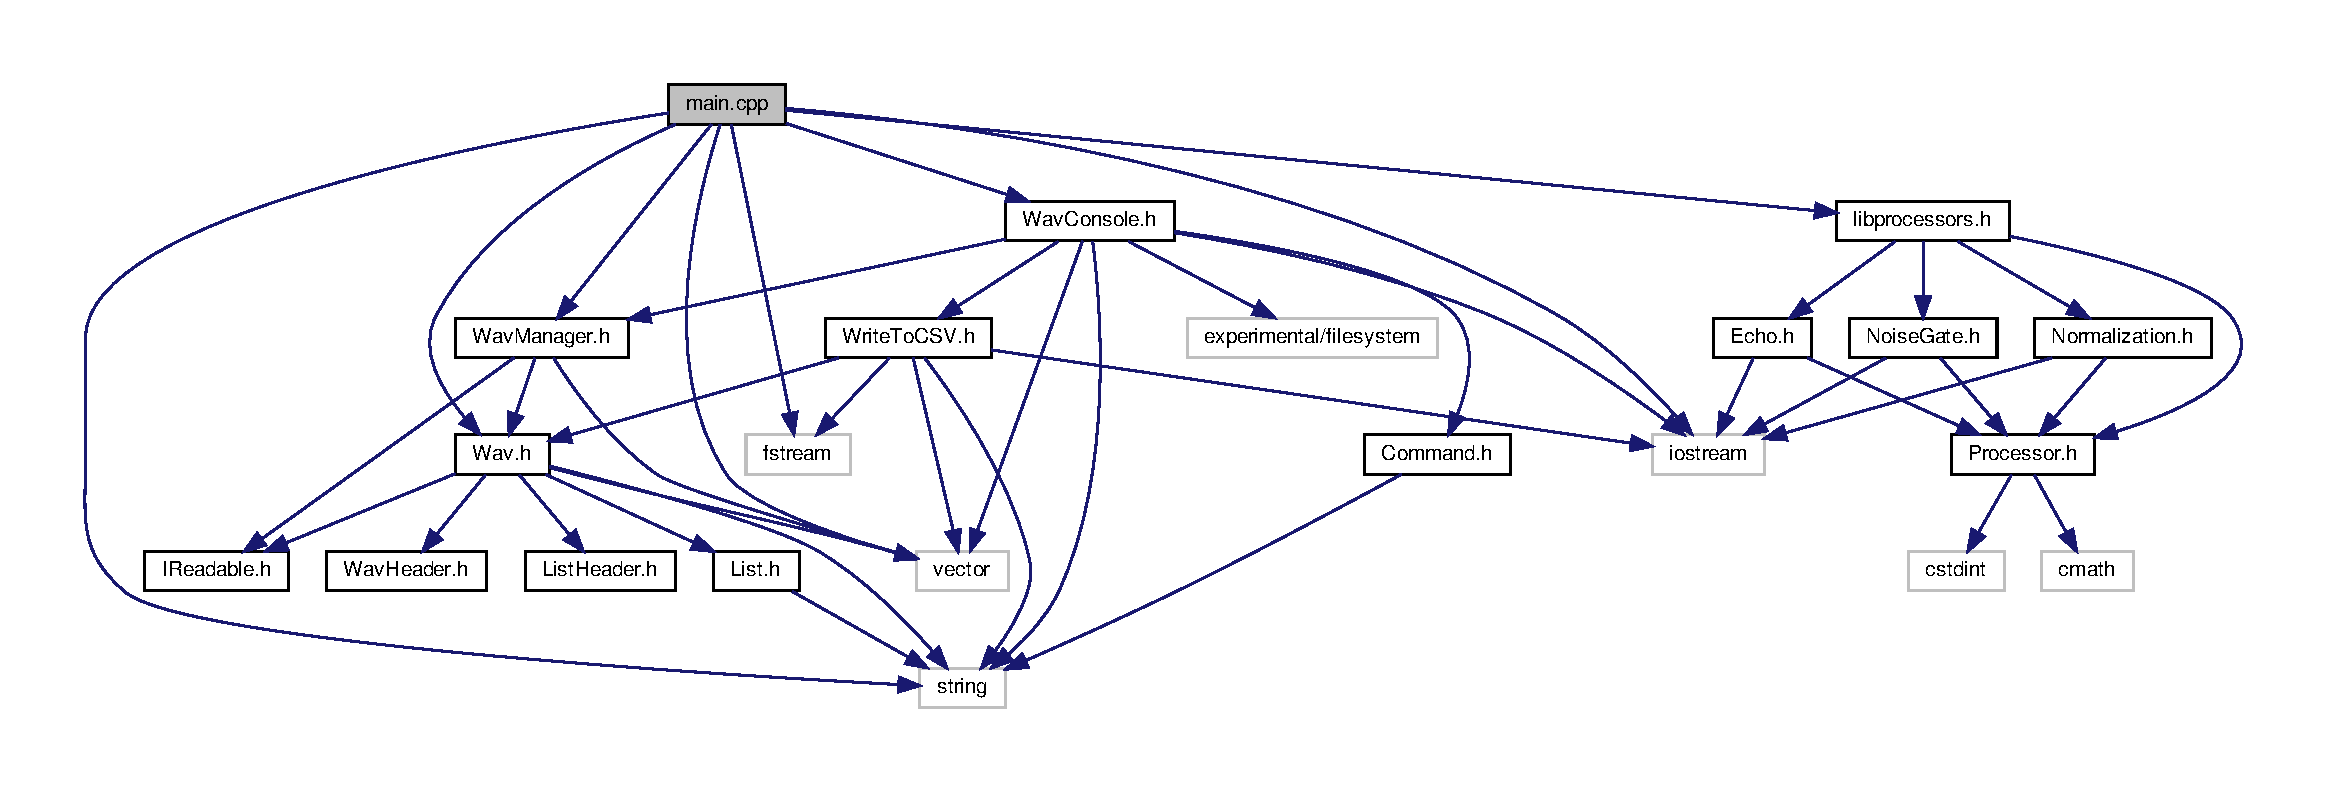
\includegraphics[width=350pt]{da/dce/main_8cpp__incl}
\end{center}
\end{figure}
\subsection*{Functions}
\begin{DoxyCompactItemize}
\item 
\mbox{\Hypertarget{main_8cpp_ae66f6b31b5ad750f1fe042a706a4e3d4}\label{main_8cpp_ae66f6b31b5ad750f1fe042a706a4e3d4}} 
int \hyperlink{main_8cpp_ae66f6b31b5ad750f1fe042a706a4e3d4}{main} ()
\begin{DoxyCompactList}\small\item\em This function initializes and runs the \hyperlink{classWavConsole}{Wav\+Console}. Most of the direct user-\/facing behavior is encapsulated within that class, so the main function is pretty minimalist. \end{DoxyCompactList}\end{DoxyCompactItemize}
\subsection*{Variables}
\begin{DoxyCompactItemize}
\item 
\mbox{\Hypertarget{main_8cpp_adf64c61a32e3b8adeb57df9dfaf3020d}\label{main_8cpp_adf64c61a32e3b8adeb57df9dfaf3020d}} 
const std\+::string {\bfseries \+\_\+8bitM} = \char`\"{}yes-\/8bit-\/mono.\+wav\char`\"{}
\item 
\mbox{\Hypertarget{main_8cpp_a21450c51782ad15cc025e77621f64fcf}\label{main_8cpp_a21450c51782ad15cc025e77621f64fcf}} 
const std\+::string {\bfseries \+\_\+8bitS} = \char`\"{}yes-\/8-\/bit-\/stereo.\+wav\char`\"{}
\item 
\mbox{\Hypertarget{main_8cpp_ad3aca47d0c41f08903bcc9a2908f4343}\label{main_8cpp_ad3aca47d0c41f08903bcc9a2908f4343}} 
const std\+::string {\bfseries \+\_\+16bitM} = \char`\"{}yes-\/16-\/bit-\/mono.\+wav\char`\"{}
\item 
\mbox{\Hypertarget{main_8cpp_a8ea0aaa1371a2fe953a1ebff73c1df27}\label{main_8cpp_a8ea0aaa1371a2fe953a1ebff73c1df27}} 
const std\+::string {\bfseries \+\_\+16bitS} = \char`\"{}yes-\/26-\/bit-\/stereo.\+wav\char`\"{}
\end{DoxyCompactItemize}

%--- End generated contents ---

% Index
\backmatter
\newpage
\phantomsection
\clearemptydoublepage
\addcontentsline{toc}{chapter}{Index}
\printindex

\end{document}
